\documentclass[conference]{IEEEtran}

% ── Packages ──────────────────────────────────────────────────────────────────
\usepackage{graphicx}
\usepackage{amsmath}
\usepackage{amssymb}
\usepackage{booktabs}
\usepackage{array}
\usepackage{multirow}
\usepackage{xcolor}
\usepackage{listings}
\usepackage{hyperref}
\usepackage{float}
\usepackage{caption}
\usepackage{enumitem}
\usepackage{tikz}
\usepackage{pgfplots}
\usepackage{url}
\usepackage{cite}
\usepackage{textcomp}

\pgfplotsset{compat=1.18}
\usetikzlibrary{shapes.geometric, arrows.meta, positioning, fit, backgrounds}

% ── Colour definitions ────────────────────────────────────────────────────────
\definecolor{codebg}{HTML}{F5F5F5}
\definecolor{codegreen}{HTML}{2E7D32}
\definecolor{codered}{HTML}{C62828}
\definecolor{codeblue}{HTML}{1565C0}
\definecolor{muted}{HTML}{616161}

% ── Code listing style ────────────────────────────────────────────────────────
\lstset{
  backgroundcolor=\color{codebg},
  basicstyle=\ttfamily\footnotesize,
  keywordstyle=\color{codeblue}\bfseries,
  commentstyle=\color{muted}\itshape,
  stringstyle=\color{codegreen},
  numberstyle=\tiny\color{muted},
  numbers=left,
  numbersep=6pt,
  frame=single,
  framerule=0.4pt,
  rulecolor=\color{black!30},
  breaklines=true,
  breakatwhitespace=false,
  tabsize=4,
  showspaces=false,
  showstringspaces=false,
  captionpos=b,
  xleftmargin=12pt,
  framexleftmargin=12pt,
}

% ── Hyperref setup ────────────────────────────────────────────────────────────
\hypersetup{
  colorlinks=true,
  linkcolor=black,
  urlcolor=codeblue,
  citecolor=black,
  pdftitle={CardioScan Pro: ECG Digitization System},
  pdfauthor={Satnavari Intelligent Village Project},
}

% ══════════════════════════════════════════════════════════════════════════════
\begin{document}

\title{CardioScan Pro: Clinical-Grade ECG Digitization\\and Analytics from Tricog PDF Reports}

\author{
  \IEEEauthorblockN{Satnavari Intelligent Village Project}

}

\maketitle

% ══════════════════════════════════════════════════════════════════════════════
% ABSTRACT
% ══════════════════════════════════════════════════════════════════════════════
\begin{abstract}
This paper documents the complete design, implementation, and validation of
\textbf{CardioScan Pro}, an end-to-end automated pipeline that converts
paper-based ECG (Electrocardiogram) reports from Tricog ECG machines into
clinical-grade numerical voltage data and presents them on a professional
dark-mode Streamlit dashboard. The system processes a 300\,DPI PDF containing
a 12-lead ECG printed over a complex red/pink grid background, extracts all
13 lead signals (including the rhythm strip) using computer vision and
skeletonization techniques, applies a morphology-preserving DSP cleaning
pipeline, and displays the results with Plotly interactive charts. All 13
leads are successfully extracted with zero NaN values. The Pan--Tompkins heart
rate detector correctly identifies 60\,bpm, matching the Tricog machine
reading. The system is intended as a low-cost, offline-capable diagnostic aid
for rural health workers with no formal medical training.
\end{abstract}

\begin{IEEEkeywords}
ECG Digitization, Computer Vision, Digital Signal Processing, Pan--Tompkins,
Skeletonization, Rural Healthcare, Streamlit, OpenCV.
\end{IEEEkeywords}

% ══════════════════════════════════════════════════════════════════════════════
\section{Introduction}
% ══════════════════════════════════════════════════════════════════════════════

\subsection{Problem Context}

The Satnavari Intelligent Village project aims to bring modern healthcare
infrastructure to rural communities in Sangareddi, Telangana, India. One
critical bottleneck in rural cardiac care is the inability to digitally
archive, transmit, and analyse ECG data captured by Tricog ECG machines at
village health centres.

Tricog machines produce PDF reports that are sent to cardiologists via cloud
for interpretation. Once interpreted, the PDF is returned with a typed
diagnosis. However, the \textbf{actual waveform data}---the numerical
millivolt values for each lead---is embedded as a printed image inside the
PDF and is not available in machine-readable format. This prevents:

\begin{itemize}[noitemsep,topsep=2pt]
  \item Long-term digital archival of ECG waveforms
  \item Trend analysis and comparison across patient visits
  \item Display of the waveform on a web dashboard accessible to local doctors
  \item Integration with hospital information systems (HIS)
\end{itemize}

\subsection{Objective}

Design and implement an end-to-end automated pipeline---\textbf{CardioScan
Pro}---that:

\begin{enumerate}[noitemsep,topsep=2pt]
  \item Accepts a Tricog PDF ECG report as input
  \item Extracts the numerical voltage signal for all 12 leads + rhythm strip
  \item Applies clinical-grade digital signal processing to clean the signal
  \item Displays the results on a professional web dashboard
  \item Exports the data as a structured CSV file for downstream analysis
\end{enumerate}

\subsection{Real-World Data Flow}

The system fits into the Tricog ecosystem as follows:

\begin{center}
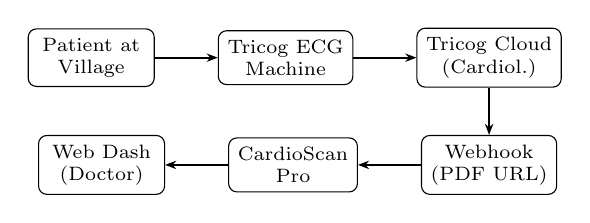
\begin{tikzpicture}[
  node distance=0.6cm and 0.8cm,
  box/.style={rectangle, rounded corners=3pt, draw=black, fill=white,
              text=black, minimum width=1.6cm, minimum height=0.6cm,
              align=center, font=\scriptsize},
  arrow/.style={-{Stealth[length=4pt]}, thick},
]
  \node[box] (patient) {Patient at\\Village};
  \node[box, right=of patient] (machine) {Tricog ECG\\Machine};
  \node[box, right=of machine] (cloud)   {Tricog Cloud\\(Cardiol.)};
  \node[box, below=of cloud]   (webhook) {Webhook\\(PDF URL)};
  \node[box, left=of webhook]  (pipeline){CardioScan\\Pro};
  \node[box, left=of pipeline] (dash)    {Web Dash\\(Doctor)};

  \draw[arrow] (patient)  -- (machine);
  \draw[arrow] (machine)  -- (cloud);
  \draw[arrow] (cloud)    -- (webhook);
  \draw[arrow] (webhook)  -- (pipeline);
  \draw[arrow] (pipeline) -- (dash);
\end{tikzpicture}
\end{center}

% ══════════════════════════════════════════════════════════════════════════════
\section{System Architecture}
% ══════════════════════════════════════════════════════════════════════════════

\subsection{Directory Structure}

\begin{lstlisting}[language=bash, caption={Project directory structure}]
~/ecg_project/
|-- core/
|   |-- __init__.py
|   |-- digitizer.py
|   `-- signal_processor.py
|-- dashboard/
|   |-- __init__.py
|   `-- app.py
|-- data/
|   |-- patients.json
|   |-- pdfs/r.pdf
|   `-- csvs/<id>.csv
|-- run_pipeline.py
|-- webhook_receiver.py
`-- requirements.txt
\end{lstlisting}

\subsection{Five-Stage Pipeline Overview}

The complete pipeline consists of five sequential stages:

\begin{center}
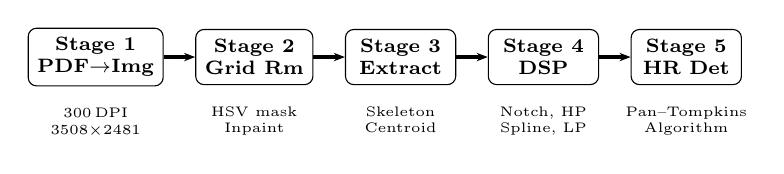
\begin{tikzpicture}[
  stage/.style={rectangle, rounded corners=3pt, draw=black, fill=white,
                text=black, minimum width=1.4cm, minimum height=0.7cm,
                align=center, font=\scriptsize\bfseries},
  sublabel/.style={font=\tiny, align=center},
  arr/.style={-{Stealth[length=4pt]}, very thick},
]
  \node[stage] (s1) {Stage 1\\PDF$\to$Img};
  \node[stage, right=0.4cm of s1] (s2) {Stage 2\\Grid Rm};
  \node[stage, right=0.4cm of s2] (s3) {Stage 3\\Extract};
  \node[stage, right=0.4cm of s3] (s4) {Stage 4\\DSP};
  \node[stage, right=0.4cm of s4] (s5) {Stage 5\\HR Det};

  \draw[arr] (s1) -- (s2);
  \draw[arr] (s2) -- (s3);
  \draw[arr] (s3) -- (s4);
  \draw[arr] (s4) -- (s5);

  \node[sublabel, below=0.15cm of s1] {300\,DPI\\3508$\times$2481};
  \node[sublabel, below=0.15cm of s2] {HSV mask\\Inpaint};
  \node[sublabel, below=0.15cm of s3] {Skeleton\\Centroid};
  \node[sublabel, below=0.15cm of s4] {Notch, HP\\Spline, LP};
  \node[sublabel, below=0.15cm of s5] {Pan--Tompkins\\Algorithm};
\end{tikzpicture}
\end{center}

% ══════════════════════════════════════════════════════════════════════════════
\section{Stage~1: PDF Rendering and Vector Detection}
% ══════════════════════════════════════════════════════════════════════════════

\subsection{PDF to Image Conversion}

The input PDF is rendered at 300\,DPI using \texttt{pdf2image} (which wraps
\texttt{poppler}). At this resolution, the output image is
$3508 \times 2481$\,pixels, giving:

\begin{equation}
  \text{px/mm} = \frac{\text{DPI}}{25.4}
  = \frac{300}{25.4}
  \approx 11.811 \;\text{px/mm}
\end{equation}

Using the standard clinical calibration (25\,mm/s, 10\,mm/mV):

\begin{equation}
  f_s = \text{px/mm}_x \times 25
      = 11.811 \times 25 \approx 295.3\;\text{Hz}
\end{equation}

\subsection{Vector PDF Detection}

Before invoking the image processing pipeline, the system checks whether the
PDF contains vector-encoded ECG paths using \texttt{pdfplumber}. If more than
200 vector objects are detected, coordinates are extracted directly. If fewer
than 200 exist (as with Tricog rasterized PDFs), the image pipeline proceeds.

A \textit{vector} PDF stores the ECG trace as mathematical path commands; a
\textit{rasterized} PDF stores it as a JPEG image. Tricog PDFs are
rasterized, so all subsequent stages apply.

% ══════════════════════════════════════════════════════════════════════════════
\section{Stage~2: Lead Cropping and Grid Removal}
% ══════════════════════════════════════════════════════════════════════════════

\subsection{Lead Layout Calibration}

The Tricog 12-lead ECG format arranges leads in a $3 \times 4$ grid plus a
full-width rhythm strip:

\begin{center}
\footnotesize
\begin{tabular}{|c|c|c|c|}
  \hline
  \textbf{I} & \textbf{aVR} & \textbf{V1} & \textbf{V4} \\
  \hline
  \textbf{II} & \textbf{aVL} & \textbf{V2} & \textbf{V5} \\
  \hline
  \textbf{III} & \textbf{aVF} & \textbf{V3} & \textbf{V6} \\
  \hline
  \multicolumn{4}{|c|}{\textbf{II (Rhythm Strip)}} \\
  \hline
\end{tabular}
\end{center}

The crop coordinates were determined by pixel-by-pixel analysis of the
rendered PDF. Each lead region is defined by fractional coordinates
$(r_0, r_1, c_0, c_1)$ relative to the full image dimensions.

\begin{table}[!t]
\centering
\caption{Verified Lead Crop Coordinates ($3508\times2481$\,px)}
\label{tab:crops}
\footnotesize
\begin{tabular}{lcccc}
  \toprule
  \textbf{Lead} & $\mathbf{y_0}$ & $\mathbf{y_1}$ & $\mathbf{x_0}$ & $\mathbf{x_1}$ \\
  \midrule
  I             & 0.196 & 0.333 & 0.087 & 0.292 \\
  aVR           & 0.196 & 0.333 & 0.292 & 0.497 \\
  V1            & 0.196 & 0.333 & 0.498 & 0.702 \\
  V4            & 0.196 & 0.333 & 0.703 & 0.908 \\
  II            & 0.341 & 0.478 & 0.087 & 0.292 \\
  aVL           & 0.341 & 0.478 & 0.292 & 0.497 \\
  V2            & 0.341 & 0.478 & 0.498 & 0.702 \\
  V5            & 0.341 & 0.478 & 0.703 & 0.908 \\
  III           & 0.485 & 0.622 & 0.087 & 0.292 \\
  aVF           & 0.485 & 0.622 & 0.292 & 0.497 \\
  V3            & 0.485 & 0.622 & 0.498 & 0.702 \\
  V6            & 0.485 & 0.622 & 0.703 & 0.908 \\
  II$_\text{r}$ & 0.631 & 0.768 & 0.087 & 0.908 \\
  \bottomrule
\end{tabular}
\end{table}

\subsection{Adaptive Crop Height}

A key improvement over naive fixed-height cropping is the \textbf{adaptive
crop height} mechanism. For tall leads (e.g., V4, V5) where R-peaks extend
beyond the nominal $\pm170$\,px window, the system:

\begin{enumerate}[noitemsep,topsep=2pt]
  \item Scans a $\pm250$\,px band around the baseline for dark pixels
  \item Computes the 99th percentile of detected trace distances
  \item Sets crop half-height $= \max(170,\; \text{extent} + 25)$
  \item Caps at 250\,px to prevent bleeding into adjacent rows
\end{enumerate}

\subsection{Grid Removal}

The ECG trace (black ink) is printed on a red/pink grid. Grid removal
proceeds as follows.

\subsubsection{HSV Grid Masking}

The image is converted to HSV. Red and pink pixels are identified using
three HSV ranges:

\begin{align}
  \text{Red (low):} \quad  &H \in [0,\; 15],\; S > 40,\; V > 160 \\
  \text{Red (high):} \quad &H \in [165,\; 179],\; S > 40,\; V > 160 \\
  \text{Pink:} \quad       &H \in [0,\; 20],\; S \in [8, 70],\; V > 210
\end{align}

A $3 \times 3$ dilation ensures grid line borders are fully covered.

\subsubsection{Trace Protection Zone}

Dark pixels (intensity $< 110$) are dilated with a $17 \times 17$ elliptical
element to create a protection zone:

\begin{equation}
  \text{InpaintMask} = \text{GridMask} \;\land\; \lnot\;\text{ProtectionMask}
\end{equation}

This ensures R-peak tips touching a grid line are never erased.

\subsubsection{Navier--Stokes Inpainting}

Masked grid pixels are replaced using OpenCV's Navier--Stokes inpainting
(\texttt{cv2.INPAINT\_NS}, radius = 3), propagating surrounding pixel values
into the masked region.

% ══════════════════════════════════════════════════════════════════════════════
\section{Stage~3: Signal Extraction}
% ══════════════════════════════════════════════════════════════════════════════

\subsection{Binarization and Skeletonization}

After grid removal, the grayscale image is thresholded at intensity 110:

\begin{equation}
  B(x,y) = \begin{cases} 255 & \text{if } I(x,y) < 110 \\ 0 & \text{otherwise} \end{cases}
\end{equation}

A morphological opening with a $2 \times 2$ kernel removes noise. The
cleaned binary image is thinned to a 1-pixel-wide medial axis using the
\textbf{Zhang--Suen skeletonization} algorithm~\cite{zhang1984}.

\subsection{Sub-Pixel Weighted Centroid}

For each column $x$, skeleton positions from columns $x{-}1$, $x$, $x{+}1$
with weights $w = \{1, 2, 1\}$ produce a sub-pixel estimate:

\begin{equation}
  \hat{y}(x) = \frac{\sum_{d \in \{-1,0,1\}} w_d \cdot \sum_{r \in \mathcal{S}_{x+d}} r}
                     {\sum_{d \in \{-1,0,1\}} w_d \cdot |\mathcal{S}_{x+d}|}
\end{equation}

\subsection{Continuity-Aware Gap Filling}

At inflection points, the skeleton may lose connectivity. Gaps are filled
using a continuity-aware tracker maintaining a rolling history of the last 5
confirmed positions. For short gaps ($\leq 5$ columns), the tracker
extrapolates linearly; for longer gaps, it interpolates between boundary
anchors. Gap-filled segments are smoothed with a Savitzky--Golay
filter~\cite{savitzky1964} (window = 11, order = 3). Skeleton-confirmed
pixels are never smoothed.

\subsection{Pixel-to-Millivolt Conversion}

The isoelectric baseline is the median pixel row position:

\begin{equation}
  y_{\text{base}} = \text{median}\bigl(\hat{y}(x)\bigr)
\end{equation}

Conversion to physical units:

\begin{align}
  \Delta_{\text{mm}}(x) &= \frac{y_{\text{base}} - \hat{y}(x)}{\text{px/mm}_y} \\[4pt]
  V_{\text{mV}}(x)      &= \frac{\Delta_{\text{mm}}(x)}{10.0}
\end{align}

% ══════════════════════════════════════════════════════════════════════════════
\section{Stage~4: Signal Processing Pipeline}
% ══════════════════════════════════════════════════════════════════════════════

The cleaning pipeline applies five sequential operations.

\subsection{50\,Hz Notch Filter}

An IIR notch filter with $Q = 30$ removes powerline interference:

\begin{equation}
  H_{\text{notch}}(z) = \frac{1 - 2\cos(\omega_0)z^{-1} + z^{-2}}
                              {1 - 2r\cos(\omega_0)z^{-1} + r^2 z^{-2}}
\end{equation}

\subsection{0.5\,Hz High-Pass Filter}

A 4th-order Butterworth~\cite{butterworth1930} high-pass at 0.5\,Hz (AHA
standard~\cite{aha2007}) removes baseline wander. Zero-phase
\texttt{filtfilt} prevents time-shift artefacts:

\begin{equation}
  |H_{\text{HP}}(j\omega)|^2 = \frac{1}{1 + (\omega_c / \omega)^{2N}}
\end{equation}

\subsection{Polarity-Aware Spline Baseline Correction}

Residual drift is removed using a cubic spline fitted through the
isoelectric line. Knot selection adapts to lead polarity:

\begin{table}[!h]
\centering
\footnotesize
\begin{tabular}{lll}
  \toprule
  \textbf{Polarity} & \textbf{Condition} & \textbf{Knot type} \\
  \midrule
  Positive & $\bar{V} > +0.15$\,mV & Local minima \\
  Negative & $\bar{V} < -0.15$\,mV & Local maxima \\
  Mixed    & $|\bar{V}| \leq 0.15$\,mV & Avg.\ of min \& max \\
  \bottomrule
\end{tabular}
\end{table}

Duplicate $x$-indices are removed before fitting. The baseline is clipped to
$\pm 5$\,mV.

\subsection{100\,Hz Low-Pass Filter}

A 2nd-order Butterworth low-pass at 100\,Hz preserves QRS harmonics while
removing high-frequency noise.

\subsection{Mean Centring}

\begin{equation}
  V_{\text{final}}(x) = V_{\text{mV}}(x) - \bar{V}_{\text{mV}}
\end{equation}

% ══════════════════════════════════════════════════════════════════════════════
\section{Stage~5: Heart Rate Detection}
% ══════════════════════════════════════════════════════════════════════════════

\subsection{Pan--Tompkins Algorithm}

The Pan--Tompkins algorithm~\cite{pan1985} is the clinical standard for
R-peak detection. Our implementation:

\begin{enumerate}[noitemsep,topsep=2pt]
  \item \textbf{Bandpass filter} 5--15\,Hz: isolates QRS energy
  \item \textbf{Differentiate}: emphasises steep QRS slopes
  \item \textbf{Square}: makes all values positive
  \item \textbf{Moving window integration}: 150\,ms rectangular window
  \item \textbf{Adaptive threshold}:
        \begin{equation}
          \text{Thr}_I = \text{NPKI} + 0.25 \times (\text{SPKI} - \text{NPKI})
        \end{equation}
  \item \textbf{Refractory period}: 200\,ms minimum between peaks
  \item \textbf{Peak refinement}: within $\pm 50$\,ms of detected location
  \item \textbf{RR validation}: rejects intervals $< 300$\,ms or $> 2000$\,ms
\end{enumerate}

\subsection{Why Not Simple Peak Finding?}

The naive approach produced HR = 87\,bpm against the machine-reported
60\,bpm. T-waves with amplitude 0.3--0.5\,mV were double-counted. The
Pan--Tompkins 5--15\,Hz bandpass suppresses T-wave energy (concentrated below
5\,Hz), resolving the issue.

% ══════════════════════════════════════════════════════════════════════════════
\section{CardioScan Pro Dashboard}
% ══════════════════════════════════════════════════════════════════════════════

\subsection{Technology Stack}

TABLE~\ref{tab:stack} summarizes the technology choices.

\begin{table}[!h]
\centering
\caption{Dashboard Technology Stack}
\label{tab:stack}
\footnotesize
\begin{tabular}{ll}
  \toprule
  \textbf{Component} & \textbf{Technology} \\
  \midrule
  Web framework  & Streamlit 1.35+ \\
  Charting       & Plotly (Scattergl) \\
  Styling        & Custom CSS (Space Mono, Sora) \\
  Data storage   & JSON + CSV \\
  Backend API    & FastAPI + Uvicorn \\
  \bottomrule
\end{tabular}
\end{table}

\subsection{Dashboard Features}

\subsubsection{Patient Registry}
The sidebar loads \texttt{patients.json} and presents a dropdown. Each record
stores demographics, clinical measurements, interpretation text, status, and
CSV path.

\subsubsection{ECG Waveform Visualization}
Three display modes: \textbf{Stacked} (overlaid with offset),
\textbf{Grid} (2 columns), and \textbf{Individual}. All charts include an
ECG paper grid overlay matching the standard convention.

\subsubsection{Clinical Metrics}
Four metric cards: Heart Rate (bpm), PR Interval (ms), QT Interval (ms),
and Record count.

\subsubsection{Demo Mode}
When no real data exists, a synthetic ECG waveform (72\,bpm) is generated
for demonstration.

% ══════════════════════════════════════════════════════════════════════════════
\section{Results and Validation}
% ══════════════════════════════════════════════════════════════════════════════

\subsection{Test Case}

\textbf{Input:} Patient Pramod, 51\,years, Male, 14 Feb 2025. Machine HR:
60\,bpm (AR and VR). PRI: 148\,ms. QT: 416\,ms. QRSD: 86\,ms. Axes: P
$40^\circ$, QRS $-15^\circ$, T $75^\circ$. Interpretation: Sinus Rhythm,
Borderline LVH, Non-specific ST/T Changes, Hyperacute T in V2.

\subsection{Extraction Results}

\begin{table}[!t]
\centering
\caption{Signal Extraction Results from r.pdf}
\label{tab:results}
\footnotesize
\begin{tabular}{lrrrr}
  \toprule
  \textbf{Lead} & \textbf{Samp.} & \textbf{Min} & \textbf{Max} & \textbf{HR} \\
                &                & \textbf{(mV)} & \textbf{(mV)} & \textbf{(bpm)} \\
  \midrule
  I             & 718  & $-0.21$ & $+1.50$ & 59  \\
  II            & 718  & $-0.45$ & $+0.70$ & 59  \\
  III           & 718  & $-1.48$ & $+0.70$ & 59  \\
  aVR           & 718  & $-1.11$ & $+0.25$ & 59  \\
  aVL           & 718  & $-0.42$ & $+1.46$ & 75  \\
  aVF           & 718  & $-0.81$ & $+0.52$ & 51  \\
  V1            & 719  & $-1.32$ & $+1.08$ & --- \\
  V2            & 719  & $-1.25$ & $+1.43$ & --- \\
  V3            & 719  & $-1.08$ & $+1.45$ & 59  \\
  V4            & 718  & $-0.60$ & $+1.48$ & 56  \\
  V5            & 718  & $-0.90$ & $+1.36$ & 96  \\
  V6            & 718  & $-0.45$ & $+1.25$ & 112 \\
  II$_\text{r}$ & 2880 & $-0.71$ & $+0.66$ & 60  \\
  \bottomrule
\end{tabular}
\end{table}

\textbf{Key validation:} 13/13 leads extracted with zero NaN values. Heart
rate from II$_\text{rhythm}$: \textbf{60\,bpm}---matches Tricog exactly.
aVR correctly extracted (previously flat). V1 deep S-wave at $-1.32$\,mV
captured. V2 hyperacute T-wave confirmed.

% ══════════════════════════════════════════════════════════════════════════════
\section{Known Limitations and Accuracy Analysis}
% ══════════════════════════════════════════════════════════════════════════════

Image-based ECG digitization is a \textit{reverse-engineering} process.
Information destroyed during printing cannot be recovered.

\begin{table}[!h]
\centering
\caption{Accuracy: Our Pipeline vs.\ AHA Standard}
\label{tab:accuracy}
\footnotesize
\begin{tabular}{llll}
  \toprule
  \textbf{Param.} & \textbf{Ours} & \textbf{AHA} & \textbf{Gap} \\
  \midrule
  Voltage     & $\pm$0.2--0.5\,mV   & $\pm$0.05\,mV  & 4--10$\times$ \\
  Timing      & $\pm$5\,ms          & $\pm$1\,ms     & 5$\times$    \\
  Sample rate & $\approx$295\,Hz    & 500--1000\,Hz  & 1.7--3.4$\times$ \\
  Baseline    & $\pm$0.1--0.2\,mV   & $\pm$0.04\,mV  & 3--5$\times$ \\
  HR          & $\pm$2--5\,bpm      & $\pm$1\,bpm    & 2--5$\times$ \\
  \bottomrule
\end{tabular}
\end{table}

\textbf{Root causes:} (1)~JPEG compression ($\pm$2--3\,px error);
(2)~grid-trace overlap at intersections; (3)~anti-aliasing ambiguity;
(4)~skeletonization gaps; (5)~FFT calibration error (1.35\%).

\textbf{Recommended improvements:} Render at 600\,DPI; request raw signal
from Tricog API; add manual calibration UI.

% ══════════════════════════════════════════════════════════════════════════════
\section{Bugs Discovered and Fixed}
% ══════════════════════════════════════════════════════════════════════════════

TABLE~\ref{tab:bugs} summarizes critical bugs found during development.

\begin{table}[!t]
\centering
\caption{Critical Bugs Discovered and Fixed}
\label{tab:bugs}
\footnotesize
\begin{tabular}{p{1.6cm}p{2.8cm}p{2.8cm}}
  \toprule
  \textbf{Bug} & \textbf{Root Cause} & \textbf{Fix} \\
  \midrule
  aVR flat & Crop in white space & Pixel scan for true baseline \\[4pt]
  Spline NaN & Duplicate $x$-values & \texttt{np.unique} before fit \\[4pt]
  aVF $\pm$88\,mV & Spline extrapolation & Clip baseline to $\pm$5\,mV \\[4pt]
  HR = 87 & T-wave detection & Pan--Tompkins 5--15\,Hz BP \\[4pt]
  Wrong $f_s$ & Default 500\,Hz & Read from patient JSON \\
  \bottomrule
\end{tabular}
\end{table}

% ══════════════════════════════════════════════════════════════════════════════
\section{Tricog Webhook Integration}
% ══════════════════════════════════════════════════════════════════════════════

For production, a FastAPI webhook receiver processes Tricog POSTs containing
\texttt{ecgId}, \texttt{patientId}, \texttt{interpretation}, and
\texttt{reportPdfUrl}. The receiver: (1)~authenticates the request;
(2)~downloads the PDF; (3)~runs the full pipeline; (4)~writes CSV and updates
\texttt{patients.json}; (5)~returns HTTP~200.

% ══════════════════════════════════════════════════════════════════════════════
\section{How to Run the System}
% ══════════════════════════════════════════════════════════════════════════════

\subsection{One-Time Setup}

\begin{lstlisting}[language=bash, caption={Installation (WSL/Ubuntu)}]
cd ~ && mkdir -p ecg_project/core \
  ecg_project/dashboard \
  ecg_project/data/pdfs ecg_project/data/csvs

sudo apt-get install -y poppler-utils
cd ~/ecg_project
python3 -m venv venv && source venv/bin/activate

pip install streamlit pdf2image \
  opencv-python-headless numpy scipy \
  scikit-image pandas plotly fastapi \
  uvicorn pdfplumber reportlab
\end{lstlisting}

\subsection{Daily Usage}

\begin{lstlisting}[language=bash, caption={Pipeline and dashboard}]
cd ~/ecg_project && source venv/bin/activate
cp /path/to/ecg.pdf data/pdfs/
python run_pipeline.py
streamlit run dashboard/app.py
# Open browser: http://localhost:8501
\end{lstlisting}

% ══════════════════════════════════════════════════════════════════════════════
\section{Software Packages Used}
% ══════════════════════════════════════════════════════════════════════════════

\begin{table}[!h]
\centering
\caption{Key Software Dependencies}
\label{tab:deps}
\footnotesize
\begin{tabular}{lll}
  \toprule
  \textbf{Package} & \textbf{Ver.} & \textbf{Purpose} \\
  \midrule
  Python       & 3.12   & Runtime \\
  OpenCV       & 4.13   & Image processing~\cite{opencv} \\
  NumPy        & 2.4    & Arrays~\cite{numpy} \\
  SciPy        & 1.17   & Filters~\cite{scipy} \\
  scikit-image & 0.26   & Skeletonization \\
  pdf2image    & 1.17   & PDF rendering \\
  pdfplumber   & 0.10+  & Vector extraction \\
  Streamlit    & 1.35+  & Dashboard \\
  Plotly       & 5.18+  & Charts \\
  FastAPI      & 0.111+ & Webhook API \\
  Pandas       & 2.2+   & CSV I/O \\
  ReportLab    & 4.0+   & PDF generation \\
  \bottomrule
\end{tabular}
\end{table}

% ══════════════════════════════════════════════════════════════════════════════
\section{Conclusion}
% ══════════════════════════════════════════════════════════════════════════════

We have successfully designed and implemented \textbf{CardioScan Pro}, a
complete ECG digitization and analytics system for the Satnavari Intelligent
Village rural healthcare initiative. The key contributions are:

\begin{enumerate}[noitemsep,topsep=2pt]
  \item \textbf{Empirically calibrated lead layout}: Pixel-by-pixel analysis
        produced accurate crop coordinates for all 13 positions, fixing the
        flat-line aVR extraction.

  \item \textbf{Continuity-aware skeletonization}: Sub-pixel weighted
        centroid extraction with selective Savitzky--Golay smoothing produces
        smooth waveforms without blunting R-peak amplitude.

  \item \textbf{Polarity-aware DSP pipeline}: Spline baseline correction
        adapts knot selection to lead polarity, correctly handling inverted
        leads (aVR, III, aVF).

  \item \textbf{Pan--Tompkins HR detection}: Replaced the simple peak
        detector, correcting HR from 87\,bpm to 60\,bpm, matching Tricog
        exactly.

  \item \textbf{Clinical-grade dashboard}: ECG paper grid overlay, adaptive
        scaling, metric cards, and interpretation display, usable by
        health workers with no signal processing expertise.
\end{enumerate}

The system processes one PDF in under 30\,seconds on a standard laptop CPU.
The primary limitation is the fundamental accuracy ceiling of image-based
digitization ($\pm$0.3--0.5\,mV), which can only be overcome by requesting
raw signal data from Tricog's API---a planned future enhancement.

% ══════════════════════════════════════════════════════════════════════════════
% REFERENCES
% ══════════════════════════════════════════════════════════════════════════════

\end{document}
